%% LyX 2.3.5.2 created this file.  For more info, see http://www.lyx.org/.
%% Do not edit unless you really know what you are doing.
\documentclass[letterpaper,oneside,spanish]{book}
\PassOptionsToPackage{vlined,linesnumbered,ruled}{algorithm2e}
\usepackage[T1]{fontenc}
\usepackage[utf8]{inputenc}
\setcounter{secnumdepth}{3}
\usepackage{pifont}
\usepackage{float}
\usepackage{booktabs}
\usepackage{algorithm2e}
\usepackage{amsmath}
\usepackage{amsthm}
\usepackage{amssymb}
\usepackage{graphicx}

\makeatletter

%%%%%%%%%%%%%%%%%%%%%%%%%%%%%% LyX specific LaTeX commands.
\pdfpageheight\paperheight
\pdfpagewidth\paperwidth

%% Because html converters don't know tabularnewline
\providecommand{\tabularnewline}{\\}

%%%%%%%%%%%%%%%%%%%%%%%%%%%%%% Textclass specific LaTeX commands.
\theoremstyle{remark}
\newtheorem{rem}{\protect\remarkname}
\theoremstyle{definition}
\newtheorem{defn}{\protect\definitionname}
\theoremstyle{plain}
\newtheorem{prop}{\protect\propositionname}

%%%%%%%%%%%%%%%%%%%%%%%%%%%%%% User specified LaTeX commands.
\usepackage{indentfirst}

\usepackage{titlesec}
\titleformat{\chapter}[display]{\bfseries\centering\larger}{\normalsize{\chaptertitlename\ \thechapter}}{0.5ex}{}[]
\titlespacing*{\chapter}{0pt}{-50pt}{20pt}
\titleformat{\section}[hang]{\bfseries\normalsize}{\thesection\ }{0pt}{}[]
\titleformat{\subsection}[runin]{\bfseries\normalsize}{\thesubsection\ }{0pt}{}[]
\titleformat{\paragraph}[runin]{\itshape\normalsize}{\theparagraph\ }{0pt}{}[]

\newtheoremstyle{myplain}{\topsep}{\topsep}{\itshape}{}{\scshape}{.}{.5em}{}
\newtheoremstyle{mydef}{\topsep}{\topsep}{\normalfont}{}{\scshape}{.}{.5em}{}
\theoremstyle{myplain}
\newtheorem{mythm}{Teorema}[]
\newtheorem{mylem}{Lema}[]
\newtheorem{myprop}{Proposición}[]
\theoremstyle{mydef}
\newtheorem{mydef}{Definición}[]
\newtheorem{myrmk}{Observación}[]
\newtheorem{myex}{Ejemplo}[]

\let\thm\mythm
\let\endthm\endmythm
\let\lem\mylem
\let\endlem\endmylem
\let\prop\myprop
\let\endprop\endmyprop
\let\defn\mydef
\let\enddefn\endmydef
\let\example\myex
\let\endexample\endmyex
\let\rem\myrmk
\let\endrem\endmyrmk

\usepackage{xpatch}
\newcommand{\proofnamefont}{\scshape}
\xpatchcmd{\proof}{\itshape}{\normalfont\proofnamefont}{}{}

\AtBeginDocument{
  \def\labelitemi{\Pisymbol{psy}{183}}
  \def\labelitemii{\Pisymbol{psy}{45}}
  \def\labelitemiii{\Pisymbol{psy}{215}}
}

\makeatother

\usepackage{babel}
\addto\shorthandsspanish{\spanishdeactivate{~<>.}}

\providecommand{\definitionname}{Definición}
\providecommand{\propositionname}{Proposición}
\providecommand{\remarkname}{Observación}

\begin{document}

\chapter*{Notación Asintótica}

La notación asintótica (también conocida como la \emph{notación de
Landau}) es una notación matemática que se utiliza para caracterizar,
por medio de una cota, la tasa de crecimiento de una función cuando
la variable independiente tiende a infinito.

\section*{Definiciones básicas}

Sea $n\in\mathbb{N}$ y sean $f:\mathbb{N}\to\mathbb{R}$ y $g:\mathbb{N}\to\mathbb{R}$
dos funciones \emph{asintóticamente positivas}; esto es, $f(n)$ y
$g(n)$ siempre son positivas a partir de algún valor de $n$. A continuación
se presentan las definiciones básicas para la notación asintótica.
\begin{rem}
En la notación asintótica, se utiliza el símbolo $=$ en lugar de
$\in$ para denotar que una función determinada pertenece a alguno
de los conjuntos que esta notación introduce.
\end{rem}
\begin{defn}[O grande]
Denotado como $O(g)$, es el conjunto de todas aquellas funciones
$f$ para las cuales existen dos constantes $c\in\mathbb{R}^{+}$
y $n_{0}\in\mathbb{N}$, tales que $0\le f(n)\leq c\cdot g(n)$ para
toda $n\geq n_{0}$. En términos simples, $f=O(g)$ denota q
\end{defn}
%
\begin{defn}[$\Omega$ grande]
Denotado como $\Omega(g)$, es el conjunto de todas aquellas funciones
$f$ para las cuales existen dos constantes $c$ y $n_{0}$, tales
que $0\le c\cdot g(n)\leq f(n)$ para toda $n\geq n_{0}$.
\end{defn}
%
\begin{defn}[$\Theta$ grande]
Denotado como $\Theta(g)$, es el conjunto de todas aquellas funciones
$f$ para las cuales existen tres constantes $c_{1},c_{2}\in\mathbb{R}^{+}$
y $n_{0}$, tales que $0\le c_{1}\cdot g(n)\leq f(n)\leq c_{2}\cdot g(n)$
para toda $n\geq n_{0}$.
\end{defn}
\begin{prop}
Se tiene que $f=\Theta(g)$ si y sólo si $f=O(g)$ y $f=\Omega(g)$.
\end{prop}
\begin{figure}[H]
\begin{centering}
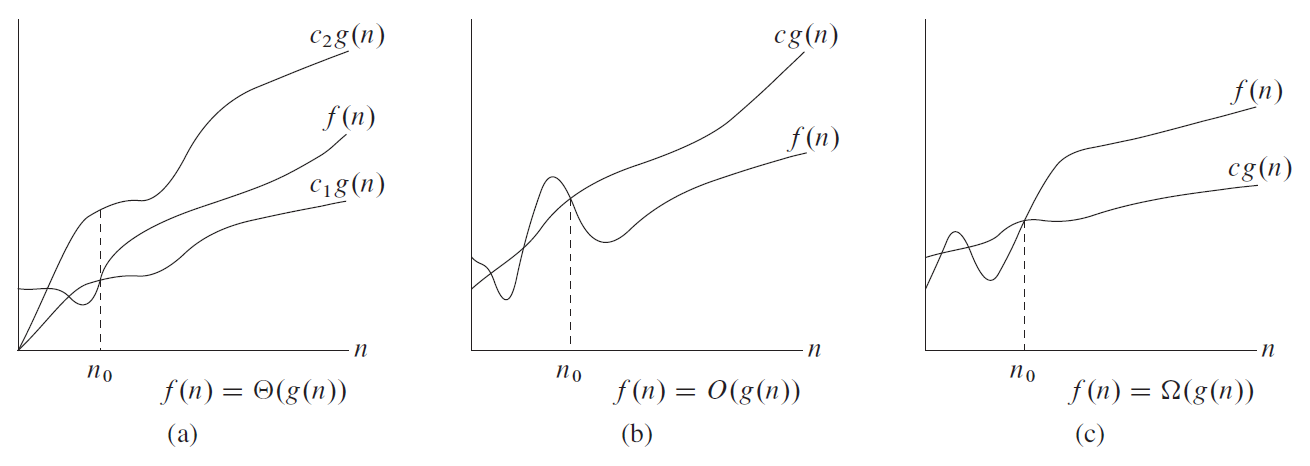
\includegraphics[width=1\textwidth]{figuras/o-grande}
\par\end{centering}
\caption{{\small{}Ejemplos de cómo interpretar gráficamente las notaciones
$\Theta$-grande, O-grande y $\Omega$-grande. (a) La notación $f=\Theta(g)$
implica que la función $g$ acota $f$ tanto por arriba como por abajo;
esto es, $g$ es una cota ajustada para $f$. (b) La notación $f=O(g)$
implica que $g$ acota $f$ por arriba; esto es, $g$ es una cota
superior para $f$. (c) La notación $f=\Omega(g)$ implica que $g$
acota $f$ por abajo; esto es, $g$ es una cota inferior para $f$.}}
\end{figure}

\begin{defn}[o chica]
Denotado como $o(g)$, es el conjunto de todas aquellas funciones
$f$ tales que, para toda constante $c$, existe una constante $n_{0}$
tal que $0\leq f(n)<c\cdot g(n)$ para toda $n\geq n_{0}$.
\end{defn}
%
\begin{defn}[$\omega$ chica]
Denotado como $\omega(g)$, es el conjunto de todas aquellas funciones
$f$ tales que, para toda constante $c$, existe una constante $n_{0}$
tal que $0\leq c\cdot g(n)<f(n)$ para toda $n\geq n_{0}$.
\end{defn}
\begin{prop}
Si $f=o(g)$, entonces $f=O(g)$.
\end{prop}
%
\begin{prop}
Si $f=\omega(g)$, entonces $f=\Omega(g)$.
\end{prop}

\section*{Trabajando con la notación asintótica}

En términos prácticos, al aplicar la notación asintótica a una expresión
algebraica, ocurren dos cosas: se eliminan los términos constantes
y los coeficientes y se consideran únicamente los términos de mayor
grado y los demás se eliminan. Intuitivamente, esto se debe a que,
conforme la variable independiente se aproxima a inifinito, la aportación
de aquellos términos que crecen más despacio se vuelve despreciable. 

\subsection*{Órdenes de crecimiento}

Al aplicar la notacion asintótica a una función, se dice que la expresión
resultante es el \emph{orden de crecimiento} (o, simplemente, \emph{orden})
de dicha función. A continuación se presentan los órdenes de crecimiento
más comunes, ordenados de aquél que crece más lento al que crece más
rápido.
\begin{enumerate}
\item \emph{Constantes}: $O(1)$
\item \emph{Logarítmicos}: $O(\log n)$
\item \emph{Radicales}: $O(\sqrt{n})$
\item \emph{Lineales}: $O(n)$
\item \emph{Súper lineales}: $O(n\cdot\log n)$
\item \emph{Cuadráticos}: $O(n^{2})$
\item \emph{Cúbicos}: $O(n^{3})$
\item \emph{Exponenciales}: $O(2^{n})$
\item \emph{Factoriales}: $O(n!)$
\end{enumerate}
\begin{rem}
Se debe tener cuidado sobre cómo se interpreta la lista anterior,
puesto que la notación asintótica puede ocultar constantes muy grandes.
Por ejemplo, a pesar de que $10^{100}n=\Theta(n)$ y $2n\cdot\log n=\Theta(n\log n)$,
se puede ver que la primera función crece muchas veces más rápido
que la segunda, para cualquier valor de $n$.
\end{rem}
\begin{figure}[tb]
\begin{centering}
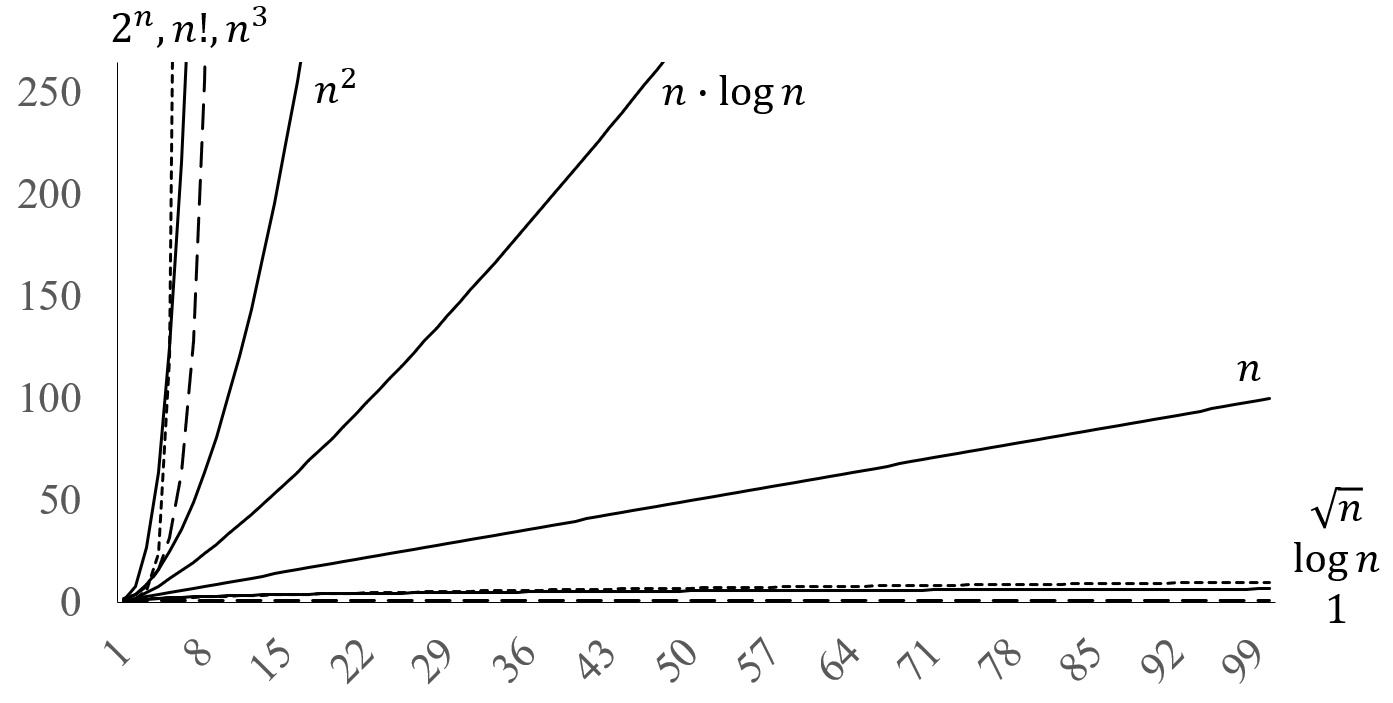
\includegraphics[width=0.8\textwidth]{figuras/ordenes}
\par\end{centering}
\caption{{\small{}Comparación gráfica de los órdenes de crecimiento más frecuentemente
utilizados en las ciencias de la computación.}}
\end{figure}


\subsection*{Propiedades aritméticas}

\paragraph{Adición}

La suma de las cotas de dos funciones está gobernada por la función
dominante.

\[
\begin{aligned}O(f)+O(g) & =O(\max\{f,g\})\\
\Omega(f)+\Omega(g) & =\Omega(\max\{f,g\})\\
\Theta(f)+\Theta(g) & =\Theta(\max\{f,g\})\\
o(f)+o(g) & =o(\max\{f,g\})\\
\omega(f)+\omega(g) & =\omega(\max\{f,g\})
\end{aligned}
\]


\paragraph{Multiplicación}

La multiplicación de una función $f$ con una constante $c$ no afecta
el comportamiento asintótico de dicha función.

\[
\begin{aligned}O(c\cdot f) & =O(f)\\
\Omega(c\cdot f) & =\Omega(f)\\
\Theta(c\cdot f) & =\Theta(f)\\
o(c\cdot f) & =o(f)\\
\omega(c\cdot f) & =\omega(f)
\end{aligned}
\]
Cuando dos funciones $f$ y $g$ se multiplican, ambas contribuyen
por igual al comportamiento asintótico de la función resultante.

\[
\begin{aligned}O(f)\cdot O(g) & =O(f\cdot g)\\
\Omega(f)\cdot\Omega(g) & =\Omega(f\cdot g)\\
\Theta(f)\cdot\Theta(g) & =\Theta(f\cdot g)\\
o(f)\cdot o(g) & =o(f\cdot g)\\
\omega(f)\cdot\omega(g) & =\omega(f\cdot g)
\end{aligned}
\]


\subsection*{Propiedades de comparación}

Muchas de las propiedades de comparación de los números reales pueden
trasladarse a funciones por medio de la notación asintótica. Una forma
intuitiva de verlo es trazando las sig. analogías:
\begin{center}
\begin{tabular}{cc}
\toprule 
Números reales & Notación asintótica\tabularnewline
\midrule
$a\leq b$ & $f=O(g)$\tabularnewline
$a\ge b$ & $f=\Omega(g)$\tabularnewline
$a=b$ & $f=\Theta(g)$\tabularnewline
$a<b$ & $f=o(g)$\tabularnewline
$a>b$ & $f=\omega(g)$\tabularnewline
\bottomrule
\end{tabular}
\par\end{center}

\paragraph{Transitividad}

Sea $h:\mathbb{N}\to\mathbb{R}$ una función asintóticamente positiva. 
\begin{itemize}
\item Si $f=\Theta(g)$ y $g=\Theta(h)$, entonces $f=\Theta(h)$.
\item Si $f=O(g)$ y $g=O(h)$, entonces $f=O(h)$. 
\item Si $f=\Omega(g)$ y $g=\Omega(h)$, entonces $f=\Omega(h)$.
\item Si $f=o(g)$ y $g=o(h)$, entonces $f=o(h)$.
\item Si $f=\omega(g)$ y $g=\omega(h)$, entonces $f=\omega(h)$.
\end{itemize}

\paragraph{Reflexividad}

Las sig. igualdades se satisfacen porque $f(n)=f(n)$ para toda $n$:

\[
\begin{aligned}f & =\Theta(f)\\
f & =O(f)\\
f & =\Omega(f)
\end{aligned}
\]


\paragraph{Simetría}

Se tiene que $f=\Theta(g)$ si y sólo si $g=\Theta(f)$.

\paragraph{Simetría traspuesta}
\begin{itemize}
\item Se tiene que $f=O(g)$ si y sólo si $g=\Omega(f)$.
\item Se tiene que $f=o(g)$ si y sólo si $g=\omega(f)$.
\end{itemize}

\paragraph{Carencia de tricotomía}

Esta es la propiedad de los números reales que dice que, dados dos
números reales $a$ y $b$, exactamente una de las sig. condiciones
debe cumplirse: $a<b$, $a=b$ o $a>b$. En otras palabras, siempre
se puede establecer una comparación relativa entre dos números reales.
La notación asintótica carece de esta propiedad, pues\emph{ }se puede
dar el caso donde no se cumple que $f=O(g)$ ni que $f=\Omega(g)$.
Por ejemplo, las funciones $f(n)=n$ y $g(n)=n^{1+\sin n}$ no se
pueden comparar utilizando notación asintótica, pues el valor del
exponente de $g$ oscila entre 0 y 2, adquiriendo todos los valores
intermedios. Esto implica que $f(n)\geq g(n)$ para algunos valores
de $n$ y que $f(n)<g(n)$ para otros.

\section*{Notas bibliográficas}
\begin{itemize}
\item Cormen T.H., Leiserson C.E., Rivest R.L. \& Stein C., ``Introduction
to Algorithms'', 3ra ed. (2009), MIT Press. Págs. 43-52.
\item Skiena S.S., ``The Algorithm Design Manual'', 2da ed. (2012), Springer.
Págs. 34-41.
\end{itemize}

\end{document}
